\subsection{Silicon Pixel Detector\label{subsec:SiPixel}} 
A new silicon pixel detector with 4 layers was installed and commissioned for the 2017 p-p run. The detector front end electronics and sensors had some improvements but for the purpose of this document can be considered equivalente to the legacy detector ones.
The whole off-detector electronics was re-designed and the FEDs are based on the
latest Xilinx FPGA technology (Virtex-7). The new firmware designs already take into account high multiplicity events. However, the performance of the FEDs needed to be evaluated in the HI multiplicity environment.

An electronics board to emulate the detector response was designed to commission the off-detector electronics. The test
board is able to receive input files with hit positions and produces at its output link a response equivalent to one of the actual FE electronics. Random and constant patterns, were injected in one FED and it was measured the throughput with a multiplicity up to 14 hits/ROC/channel. It corresponds to a multiplicity expected in pp collision with PU = 500. Figure \ref{fig:pixelFED} shows the results of the test. A rate of ~ 44 kHz at L1 can be archived in this condition. Very central PbPb events have a multiplicity equivalent of pp collisions with PU=300. More details on the test performed can be found in the presentation \cite{pixelFEROLThroughput}.

It is important to bare in mind that in case of Pb-Pb collisions, not only the average multiplicity should be considered but the peak multiplicity associated to the single event. The buffer present in the FPGA should be adjusted accordingly. During the Xe-Xe run collected the 12th of October, the buffer size was adjusted passing from 520 to 982 hits/event/channel. Also if central Xe-Xe events have a multiplicity that is 30 \% lower respect to Pb-Pb central events, the Xe-Xe run was a good test to verify the functionality of the new pixel FEDs on high multiplicity environment. 

In order to complete the studies and fully validate the FED operations also for Pb-Pb collisions, it is planned to inject Pb-Pb simulated data into the system. The test could underline bottlenecks not seen up to now. 


\begin{figure}[htbp]
\begin{center}
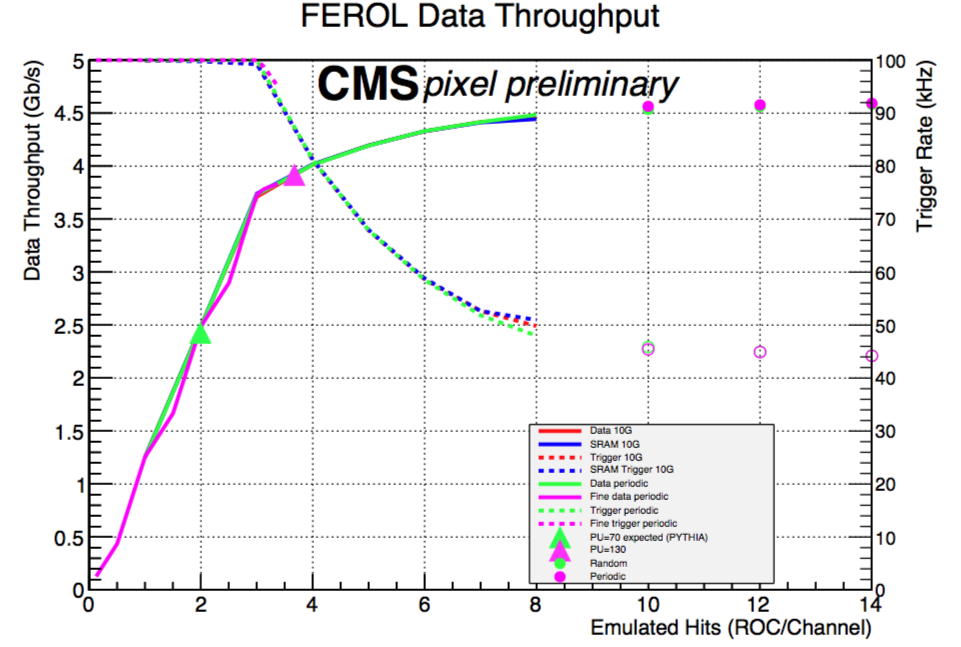
\includegraphics[width=.60\textwidth]{figures/PixelFEROLDataThroughput.png}
\caption{}
\label{fig:pixelFED}
\end{center}
\end{figure}

 

 
